\documentclass[a4paper]{article}

\usepackage[margin=1.25in]{geometry}
\usepackage{fancyhdr}
\usepackage{enumitem}
\usepackage{tabularx}
\usepackage{float}
\usepackage{subcaption}
\usepackage{array}
\usepackage{graphicx}

\usepackage[hidelinks]{hyperref}
\hypersetup{
    colorlinks=true,
    linkcolor=blue,
    filecolor=blue}

\begin{document}

\begin{titlepage}
    \thispagestyle{fancy}
    \renewcommand{\headrulewidth}{0pt}
    \begin{center}
        \vspace*{2cm}

        \LARGE\textbf{University of North Carolina at Charlotte\\
                        Department of Electrical and Computer Engineering}
        
        \vspace*{4cm}

        Homework Report $\# 3$ \\
        \Large\textbf{ECGR 4106 - Real-Time Machine Learning} \\
        
        \noindent\rule{14cm}{0.4pt}

        \vspace*{3cm}

        Name: Govind Menon \\
        Student ID: 801371478 \\
        Date: July 1, 2026 \\
        GitHub: \href{https://github.com/pGovm/introToDL.git}{pGovM/introToDL}

    \end{center}
\end{titlepage}

\section{\textbf{\textbf{Hyper Parameters}}}
These hyperparameters were shared in all 3 problems 

\begin{itemize}
    \item Hidden Size: 128
    \item Epochs: 50
    \item Learning Rate: 0.001
    \item Maximum Length of Sentence: 100
    \item Batch Size: 1
    \item Train/Val Split: 80/20
    \item Random Seed: 42
\end{itemize}

\section*{\textbf{Problem 1}}
\textbf{Objective:} Establish a baseline model for English-to-French translation using sequence-to-sequence modeling.

As specified, I used a GRU-based encoder-decoder network for my baseline architecture. After training the model, I got the following evaluation curves:

\begin{figure}[H]
    \centering
    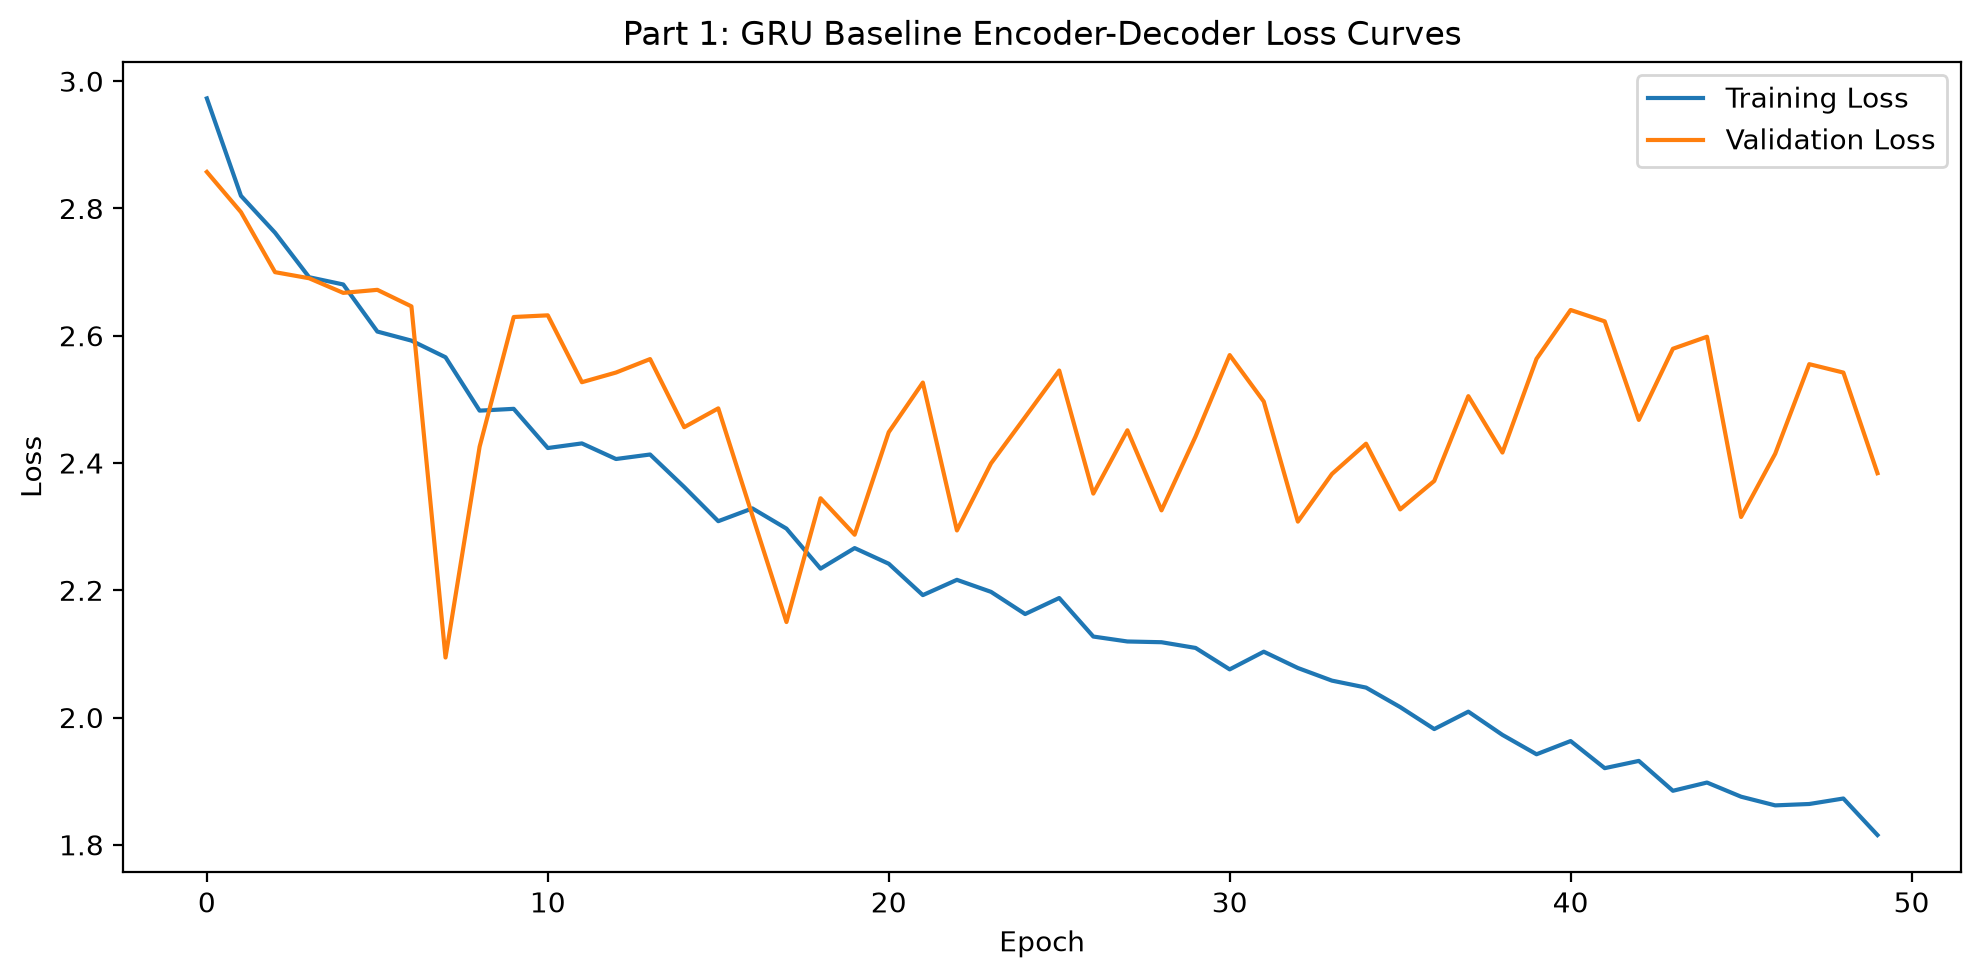
\includegraphics[width=\linewidth]{../../hw3/output/p1/data/baseline_loss_curves.png}
    \caption{\textbf{Evaluation Curves for Baseline English-to-French translation}}
    \label{fig:baseLineEval}
\end{figure}

In this graph we can see that the validation loss is slowly increasing after the 20th or so epoch while the training loss steadily decreases. This means that that the model is overfitting the data and that memorization is taking place during the training of the model. This is more pronounced when the model is trained for 100 epochs as shown below.

\begin{figure}[H]
    \centering
    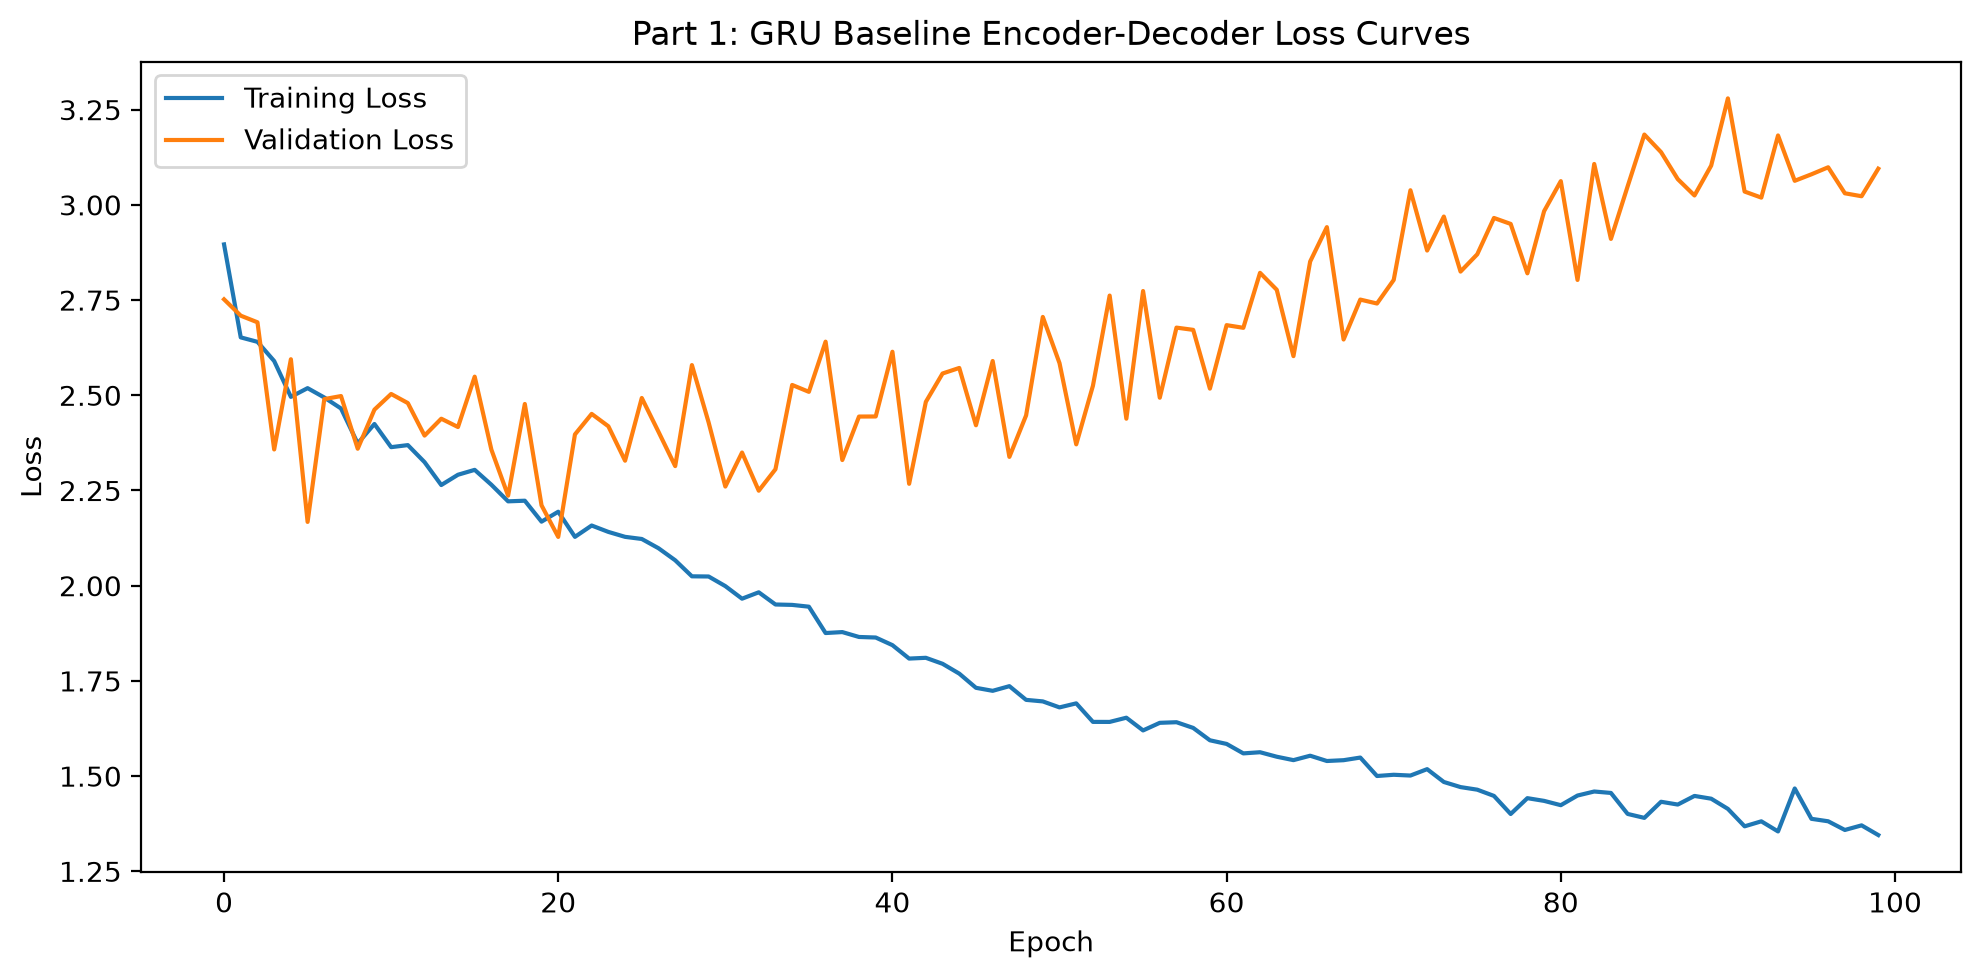
\includegraphics[width=\linewidth]{../../hw3/output/p1/data/baseline_loss_curves_overfit.png}
    \caption{\textbf{Evaluation Curves for Baseline English-to-French translation}}
    \label{fig:baseLineEvalOverFit}
\end{figure}

The above graph further enforces the notion that the model is memorizing and has stopped learning early in the training process. This also means that the dataset is not large enough for the model to be able to properly train as the gap between training and validation loss is increasing with the increasing number of epochs.

The following are the required metrics to be calculated to measure the overall accuracy of the trained models:
\begin{enumerate}
    \item \textbf{Traditional Sequence-Based Accuracy}: 0\%
    \item Validation BLEU-4 Score: 0.1359
\end{enumerate}

And when fed a couple English sentences this was the resulting translation:
\begin{figure}[H]
    \centering
    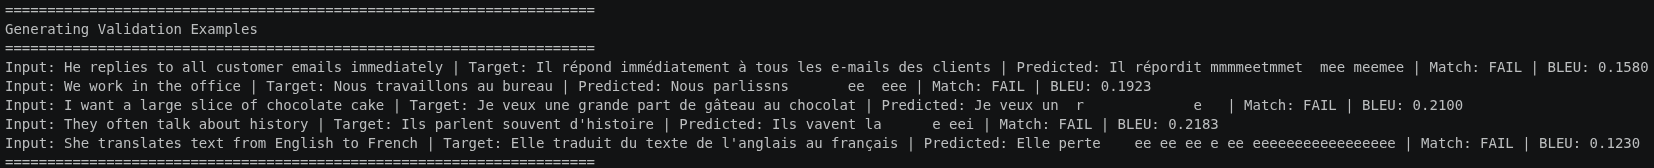
\includegraphics[width=\linewidth]{../../hw3/output/p1/qualAnalysis.png}
    \caption{\textbf{Qaulitative Analysis for Baseline English-to-French translation}}
    \label{fig:baseLineQual}
\end{figure}

From the validation BLEU score and the qualitative analysis performed we can see that the model, while it translates the first word properly has trouble in choosing the right word for a given context and sometimes even repeats itself in a loop. The traditional sequence-based accuracy is not a point of concern as all this implies is there has not been a perfect sentence translation yet.

\section*{\textbf{Problem 2}}
\textbf{Objective}: Study the performance bottleneck of a basic sequence-to-sequence model can be alleviated by implementing an attention mechanism.
For this architecture, the encoder remains the same as the previous question. The main difference is in the decoder where the attention mechanism is implemented. The Bahdanau attention mechanism is being used here as can be seen in the AttnDecoder() class where I am concatenating the hidden state and embedding before passing it through a linear layer. In addition to these class changes, a lot of the helper functions also changed as the encoder loop collects intermediate encoder outputs into a tensor instead of the just the final hidden state which is then sent to the decoder loops and then to the decoder class during training and validation.

After training the model on the same hyperparameters as the previous problem, I obtained the following evaluation curves:

\begin{figure}[H]
    \centering
    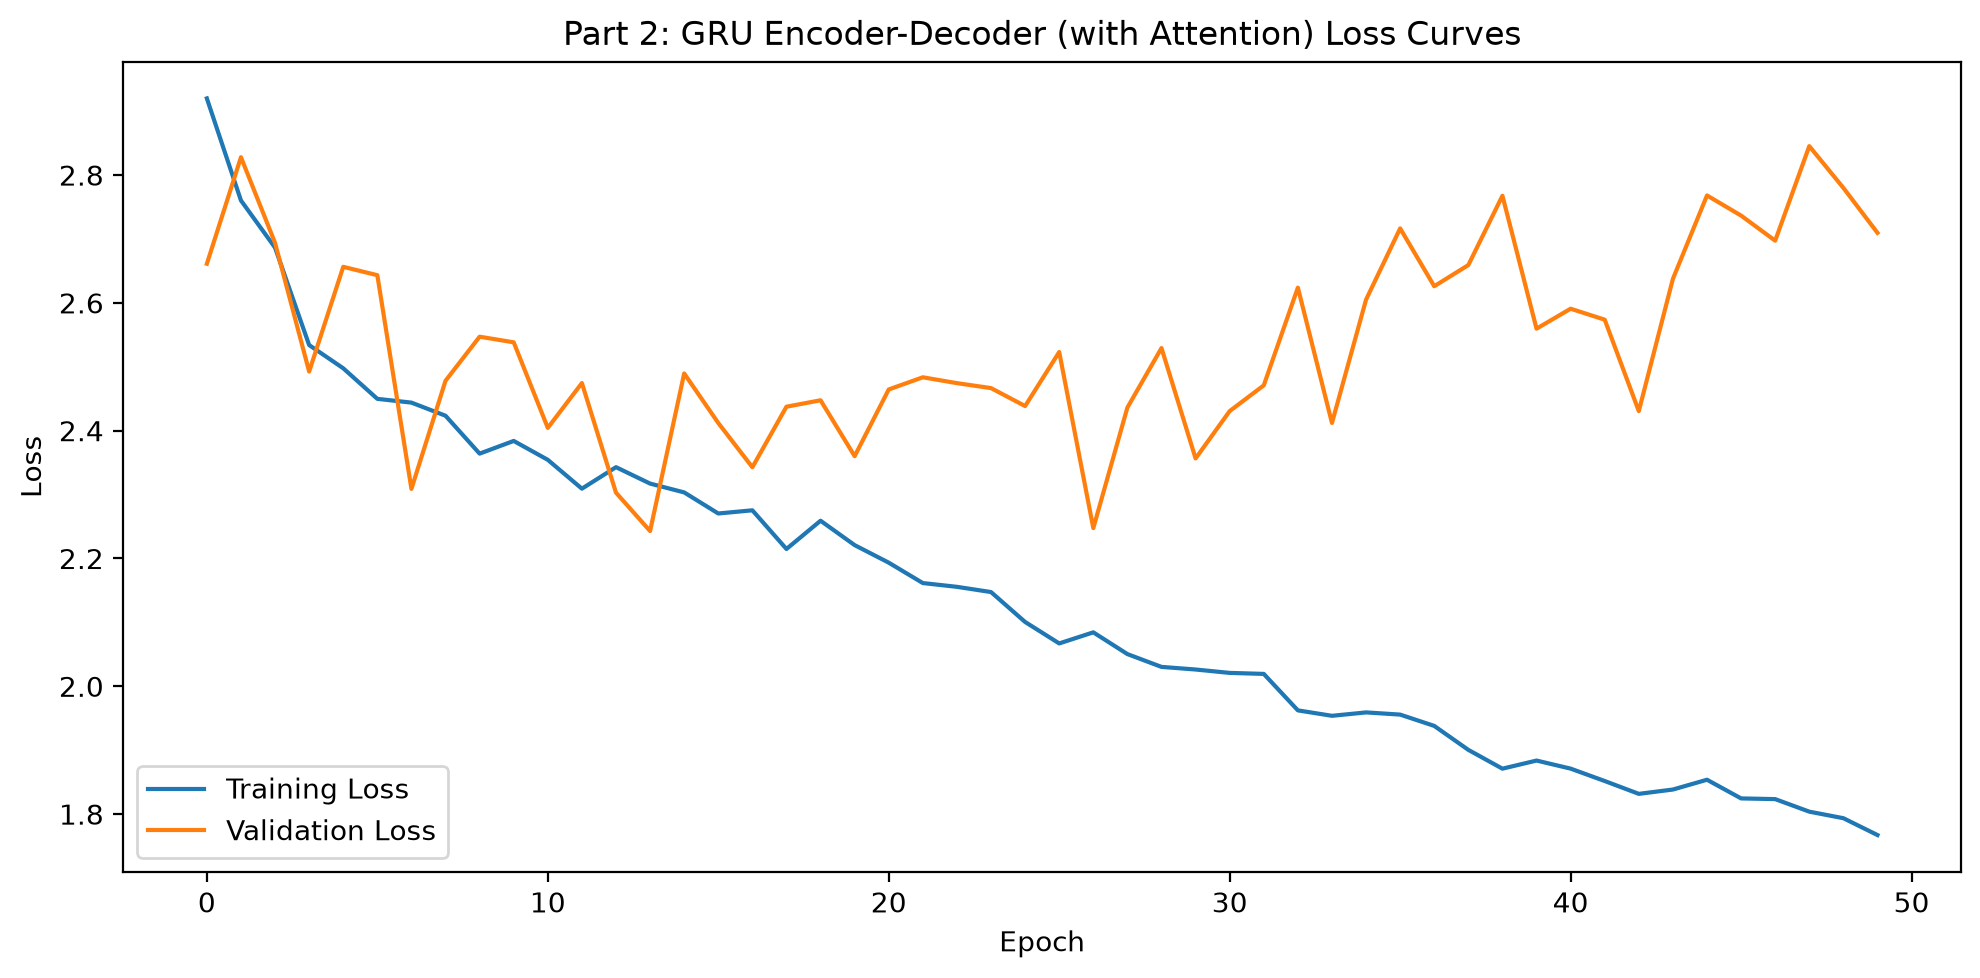
\includegraphics[width=\linewidth]{../../hw3/output/p2/data/attention_loss_curves.png}
    \caption{\textbf{Evaluation Curves for English-to-French Translation with Attention}}
    \label{fig:attnEval}
\end{figure}

This curve looks similar to Figure \ref{fig:baseLineEval} but the final training and validation losses are further apart and the first one has a lower validation loss. This implies that the model with attention, is overfitting more as the upward trend of the validation loss is more pronounced. A possible explanantion for this could the addition of extra parameters in the AttnDecoder class that is not present in the baseline Decoder class.

After evaluating the network on the validation split, the following metrics were produced:
\begin{enumerate}
    \item \textbf{Traditional Sequence-Based Accuracy}: 0\%
    \item Validation BLEU-4 Score: 0.1568
\end{enumerate}
The higher BLEU score indicates that, while not a significant difference, the attention model has still improved the translation quality. Even though the tradition accuracy is still a 0, the BLEU is higher because more parts of the translated sentence produced by the network is starting to match the target translated sentence which shows that we are taking a step in the right direction by adding the attention mechanism instead of just using the baseline as we did in Problem 1 before. Below are the results of the required qualitative tests that were run.

\begin{figure}[H]
    \centering
    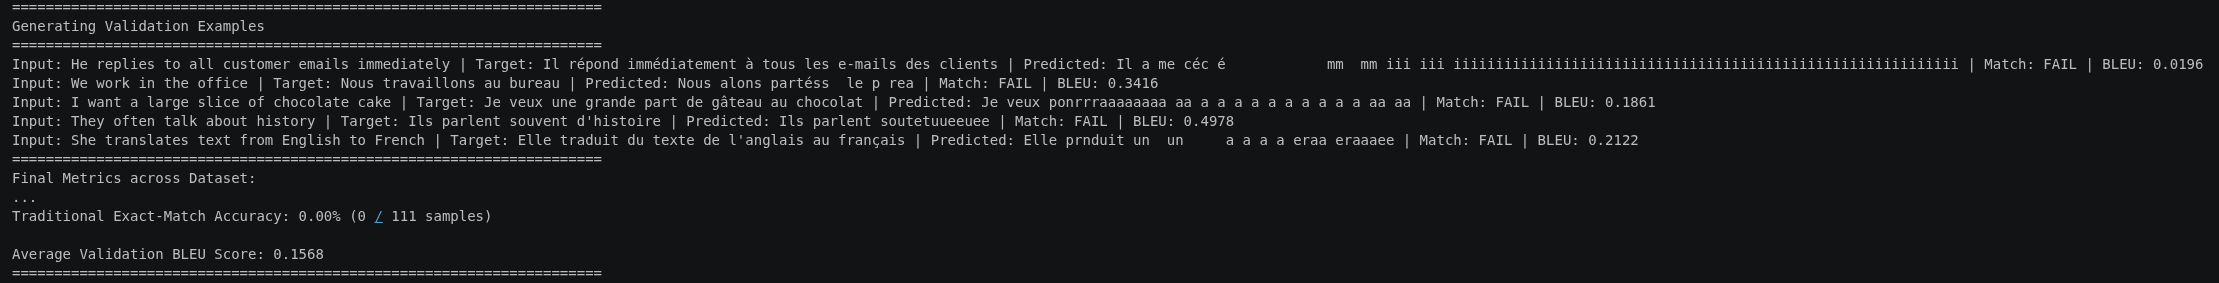
\includegraphics[width=\linewidth]{../../hw3/output/p2/data/qualAnalysis.png}
    \caption{\textbf{Qualitative Analysis for English-to-French Translation with Attention}}
    \label{fig:attnQualEval}
\end{figure}

\begin{figure}[H]
    \centering
    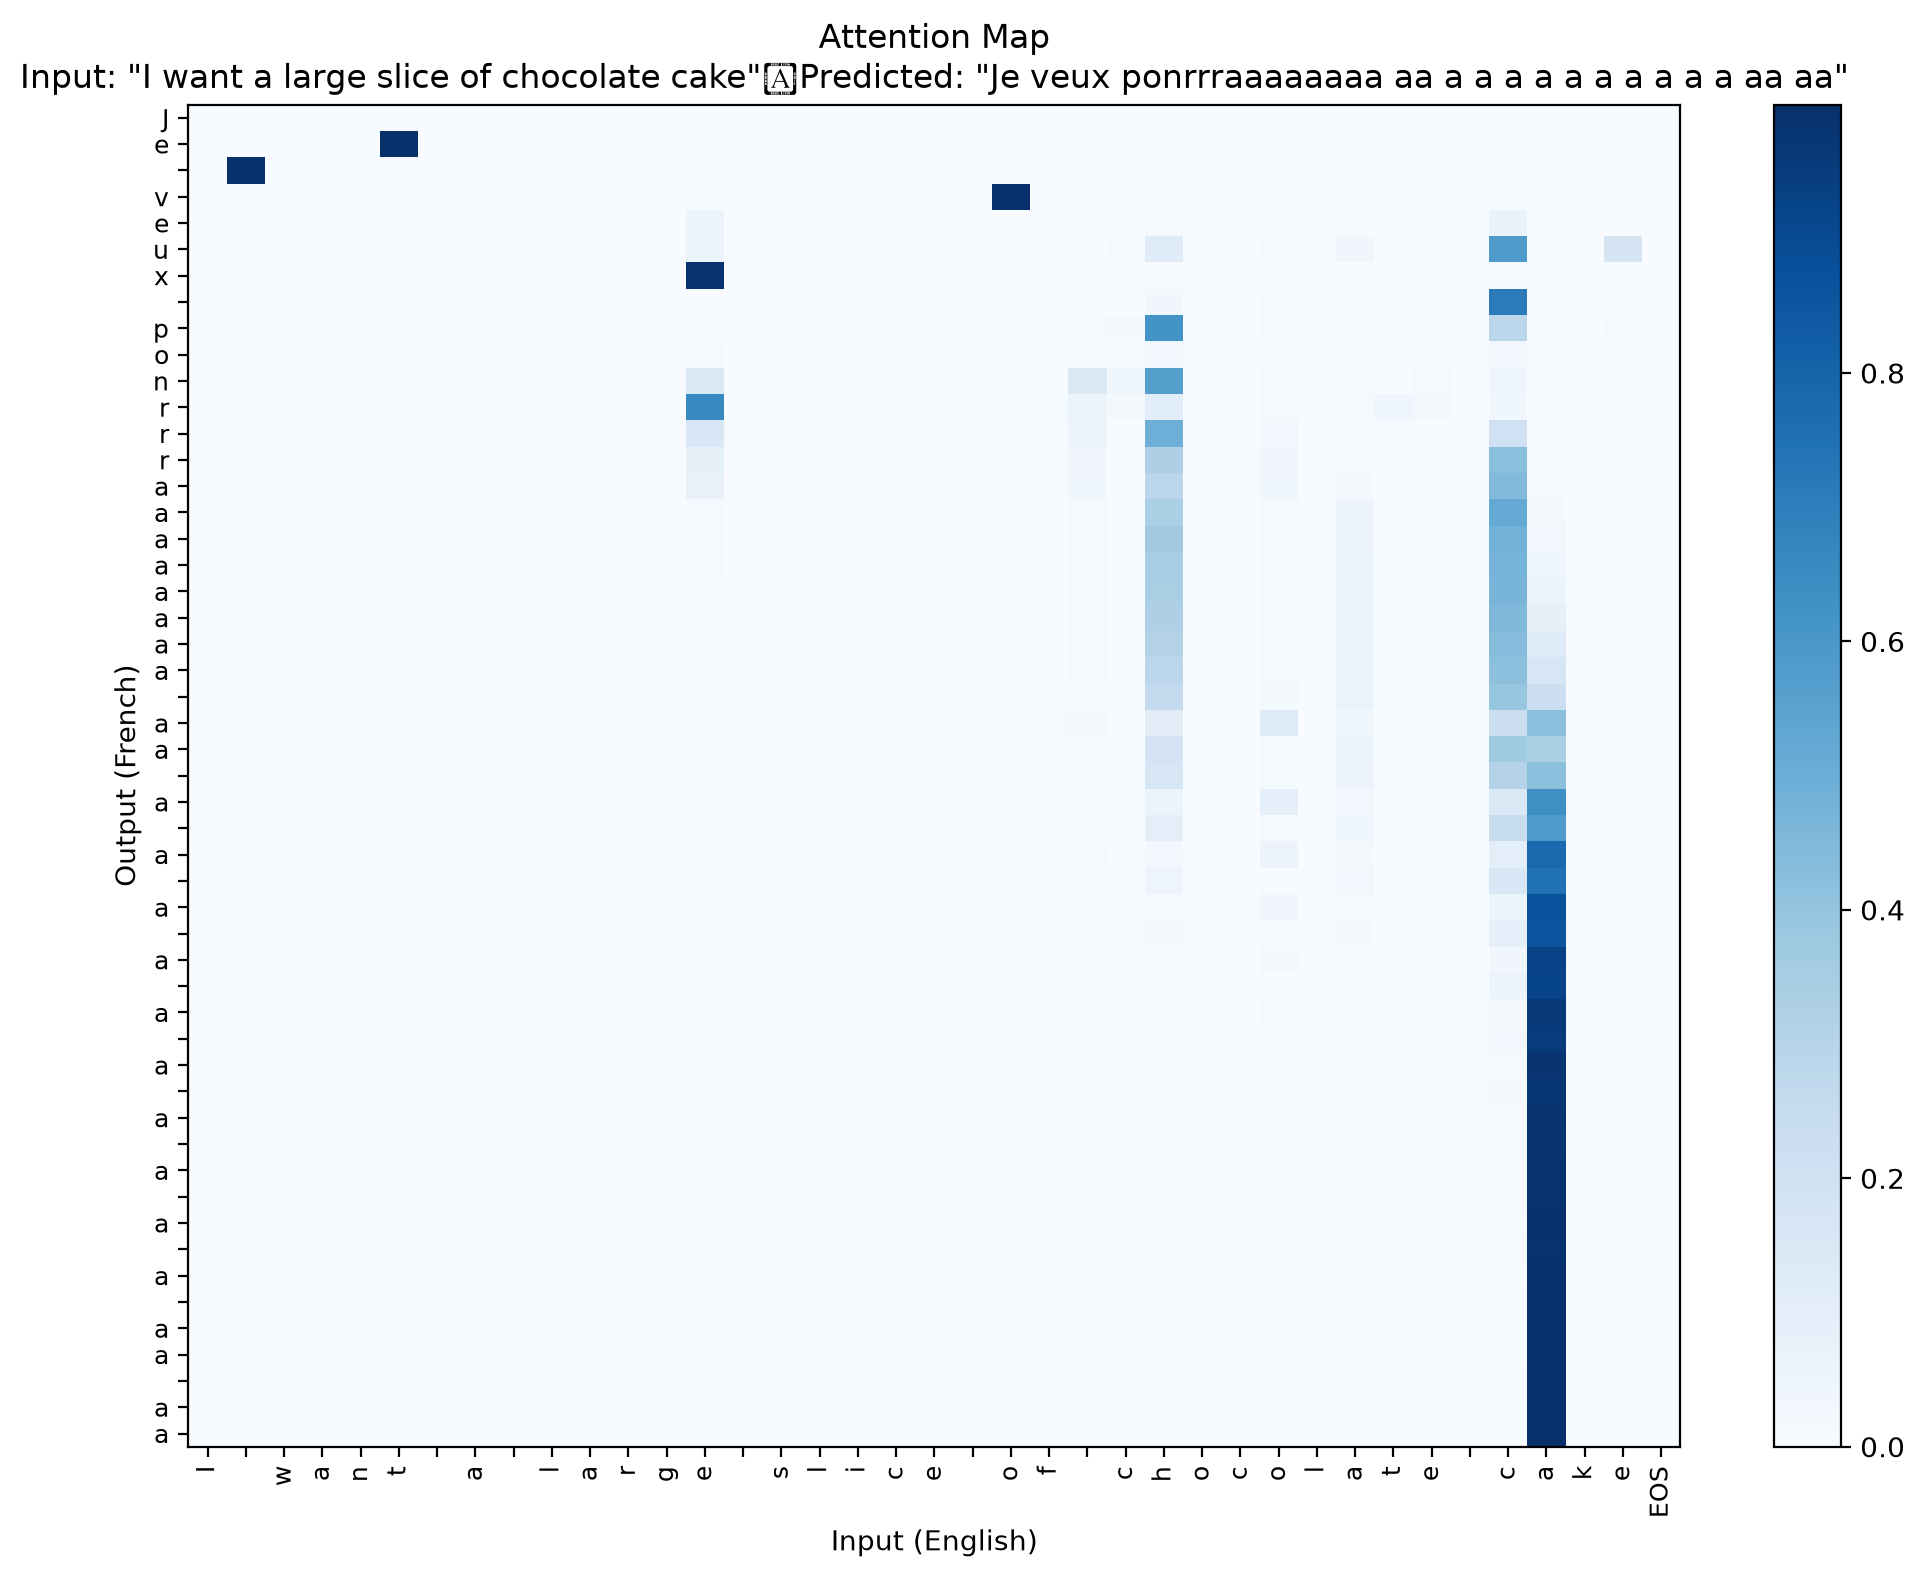
\includegraphics[width=\linewidth]{../../hw3/output/p2/data/attn_map_3.png}
    \caption{\textbf{Attention Map for English-to-French Translation with Attention}}
    \label{fig:attnMap1}
\end{figure}

\begin{figure}[H]
    \centering
    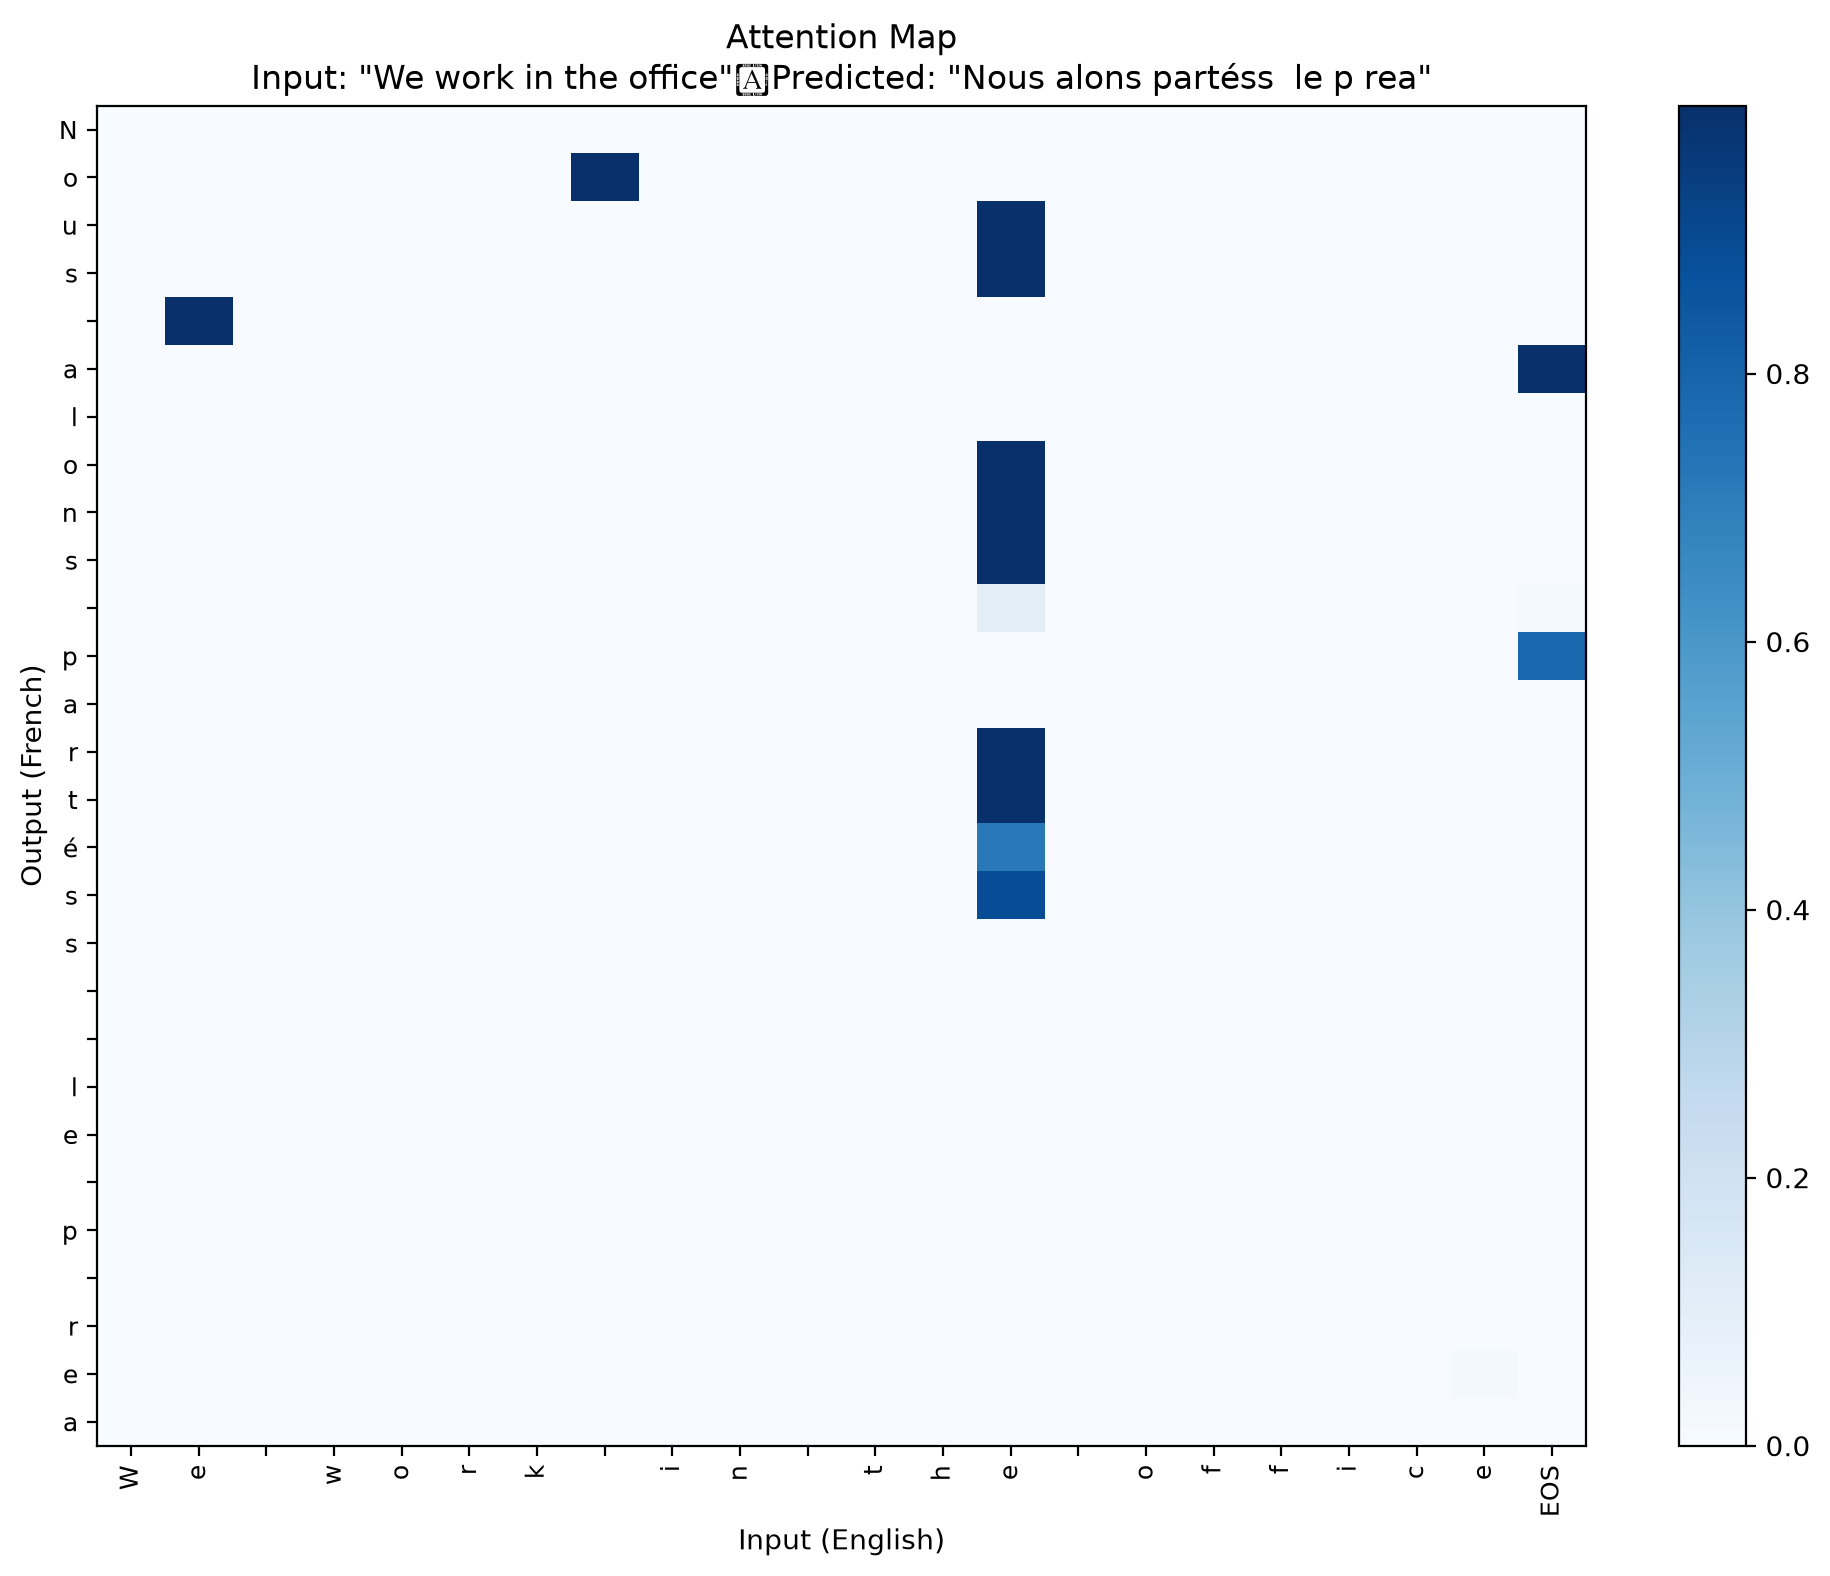
\includegraphics[width=\linewidth]{../../hw3/output/p2/data/attn_map_2.png}
    \caption{\textbf{Attention Map for English-to-French Translation with Attention}}
    \label{fig:attnMap2}
\end{figure}

In these attention maps we can see that the pattern is not diagonal but also not evenly spread. This indicates that while proper learning has not been conducted, the network was still able to link certain words or letters between the English and French languages that it knows to pay more attention to. Which is the same story told by the BLEU score.

\section*{\textbf{Problem 3}}
\textbf{Objective}: Evaluate problems 1 and 2 and change the translation target from French to English.
There were no major changes to either architecture for this section of the homework. The only change was that the dsataset used was reversed to enable french-to-english translation training.

For the baseline architecture, the following evaluation curves were plotted:

\begin{figure}[H]
    \centering
    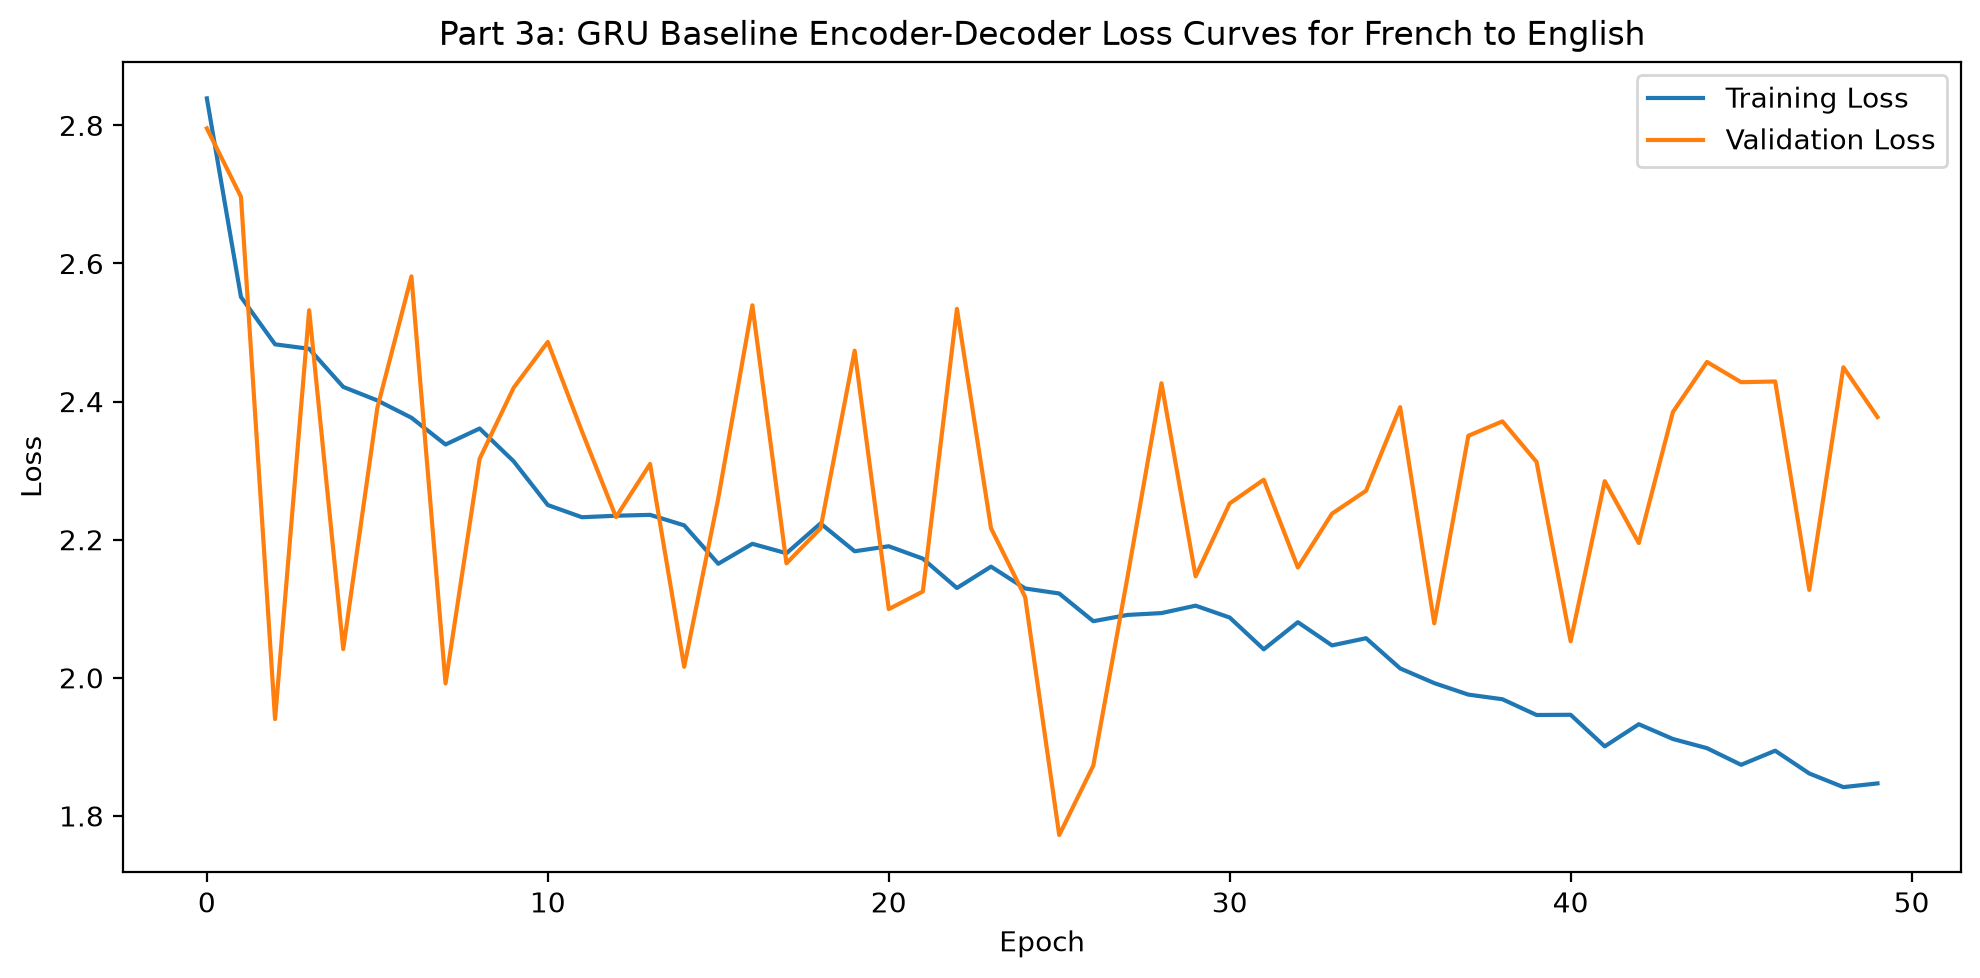
\includegraphics[width=\linewidth]{../../hw3/output/p3/baseline_loss_curves_reversed.png}
    \caption{\textbf{Evaluation Curves for Baseline French-to-English Translation}}
    \label{fig:reverseBaselineEval}
\end{figure}

In comparison to the original baseline curves, these seem to indicate a higher validation and training loss for the reversed dataset but the curves seem to be more aligned or seem to indicate less overfitting which means that the reversed model was able to learn more than the original network. The same should be reflected in the BLEU scores that we will look at in a moment.

\begin{figure}[H]
    \centering
    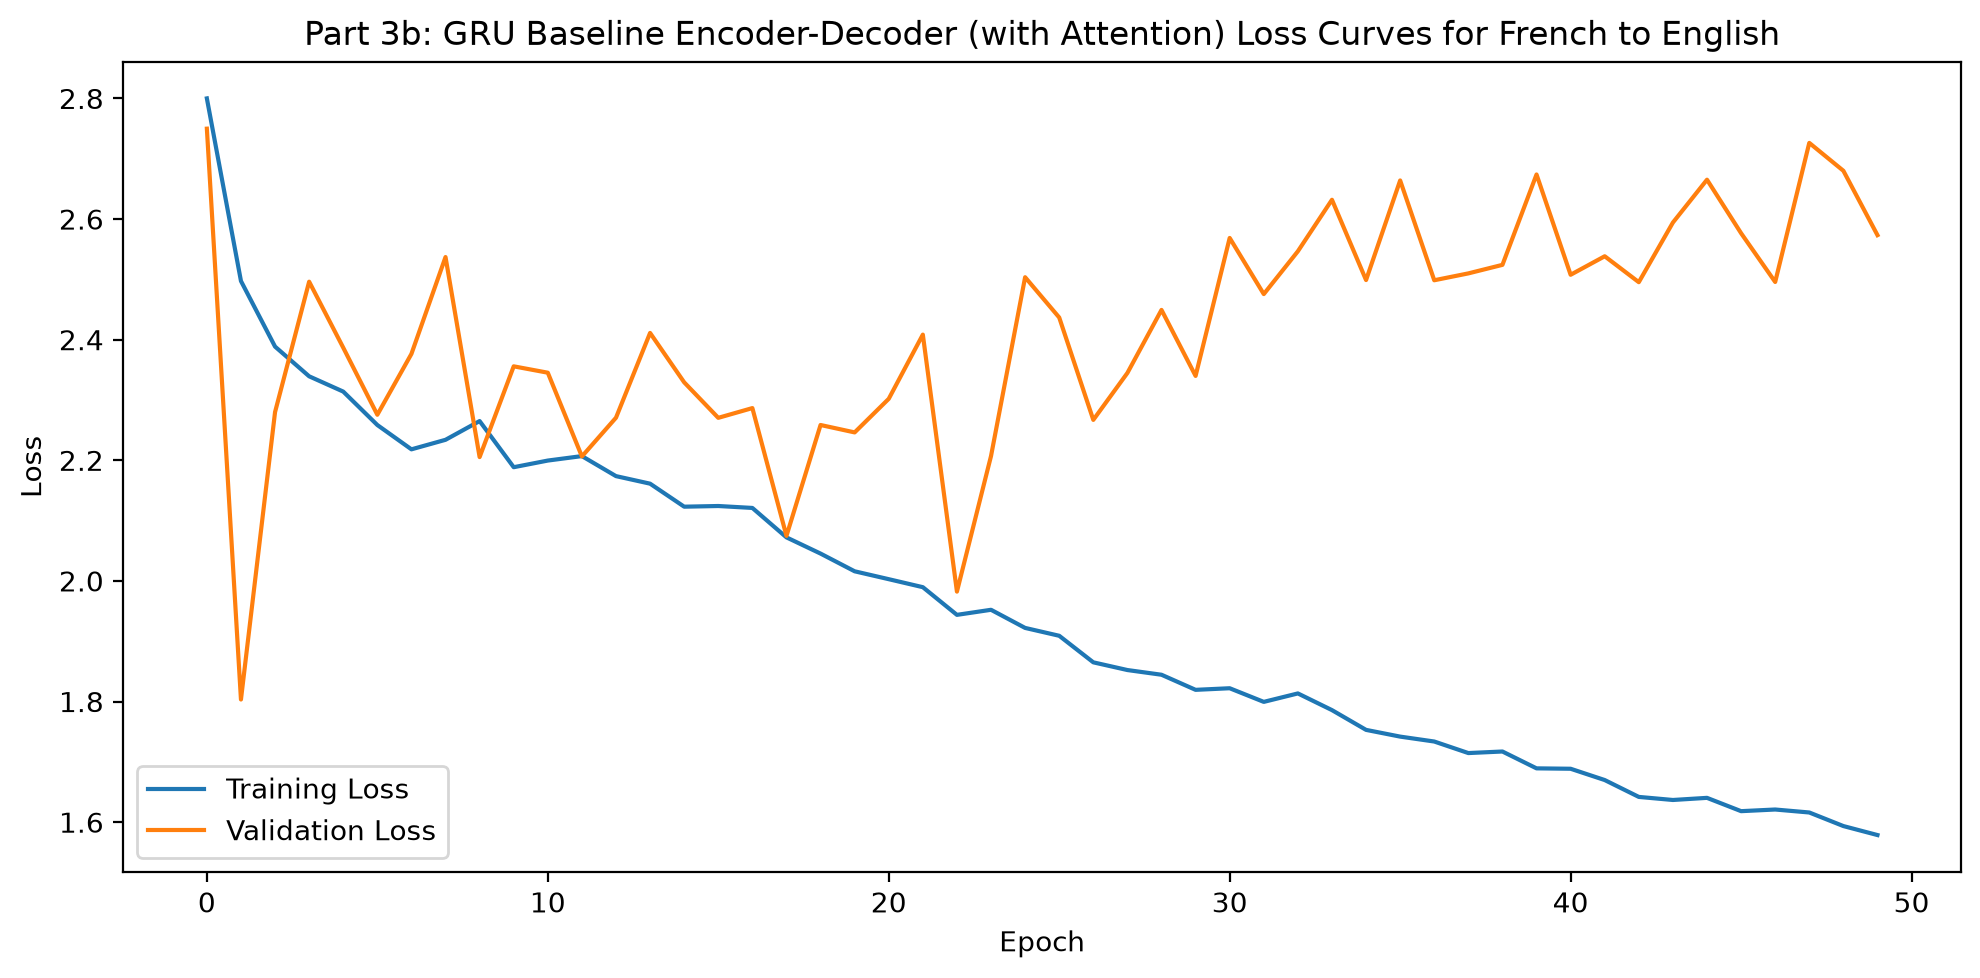
\includegraphics[width=\linewidth]{../../hw3/output/p3/attention_loss_curves.png}
    \caption{\textbf{Evaluation Curves for French-to-English Translation with Attention}}
    \label{fig:reverseAttnEval}
\end{figure}

While these may not be as pronounced as the baseline evaluation curves, it can still be seen how the reversed evaluation curves for the network with attention seems to overfit less and thus indicates more learning took place in comparison to the original attention network dataset.

These are the metrics for both baseline and attention networks:
\begin{enumerate}
    \item \textbf{Baseline Metrics}:
            \begin{itemize}
                \item Traditional Sequence-Based Accuracy: 0\%
                \item Validation BLEU-4 Score: 0.1257
            \end{itemize}
    \item \textbf{Attention Metrics}:
            \begin{itemize}
                \item Traditional Sequence-Based Accuracy: 0\%
                \item Validation BLEU-4 Score: 0.1578
            \end{itemize}
\end{enumerate}

Even though the baseline evluation curves indicate that the network with the reversed dataset has less overfitting, the BLEU score shows the opposite. A possible reason for this could be that even though the latter network learned more, the increased contexts caused the model to misinterpret the intent of the sentence. Moving on, the attention network with the reversed dataset has a significantly higher BLEU score than the original network. This metric confirms what was said previously that the current model has less overfitting and, as such, was able to learn more.

These were the qualitative tests that were run:

\begin{figure}[H]
    \centering
    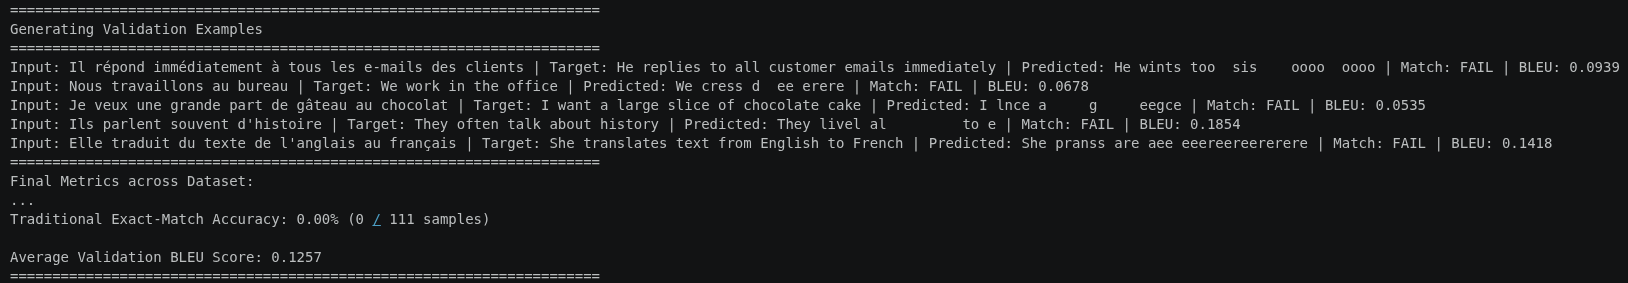
\includegraphics[width=\linewidth]{../../hw3/output/p3/reverseBaselineQualAnalysis.png}
    \caption{\textbf{Qualitative Analysis for Baseline French-to-English Translation}}
    \label{fig:reversedBaselineQualEval}
\end{figure}

\begin{figure}[H]
    \centering
    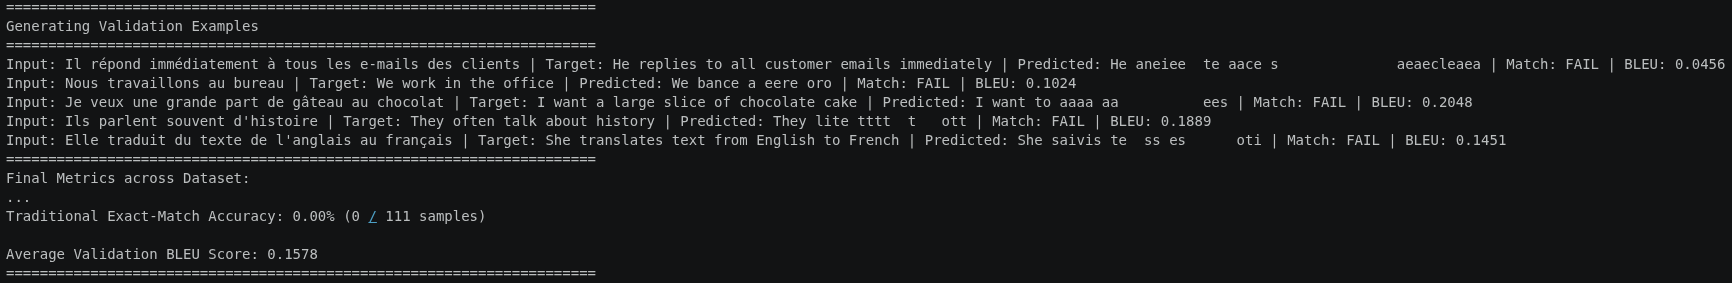
\includegraphics[width=\linewidth]{../../hw3/output/p3/reverseAttnQualAnalysis.png}
    \caption{\textbf{Qualitative Analysis for French-to-English Translation with Attention}}
    \label{fig:reversedAttnQualEval}
\end{figure}

Something both these qualitative tests have in common are that the first word or letter is always right and from there the model struggles to translate the rest of the sentence however, the occurrence of repeating letters has drastically decreased although some of these words are still unintelligible.

\begin{figure}[H]
    \centering
    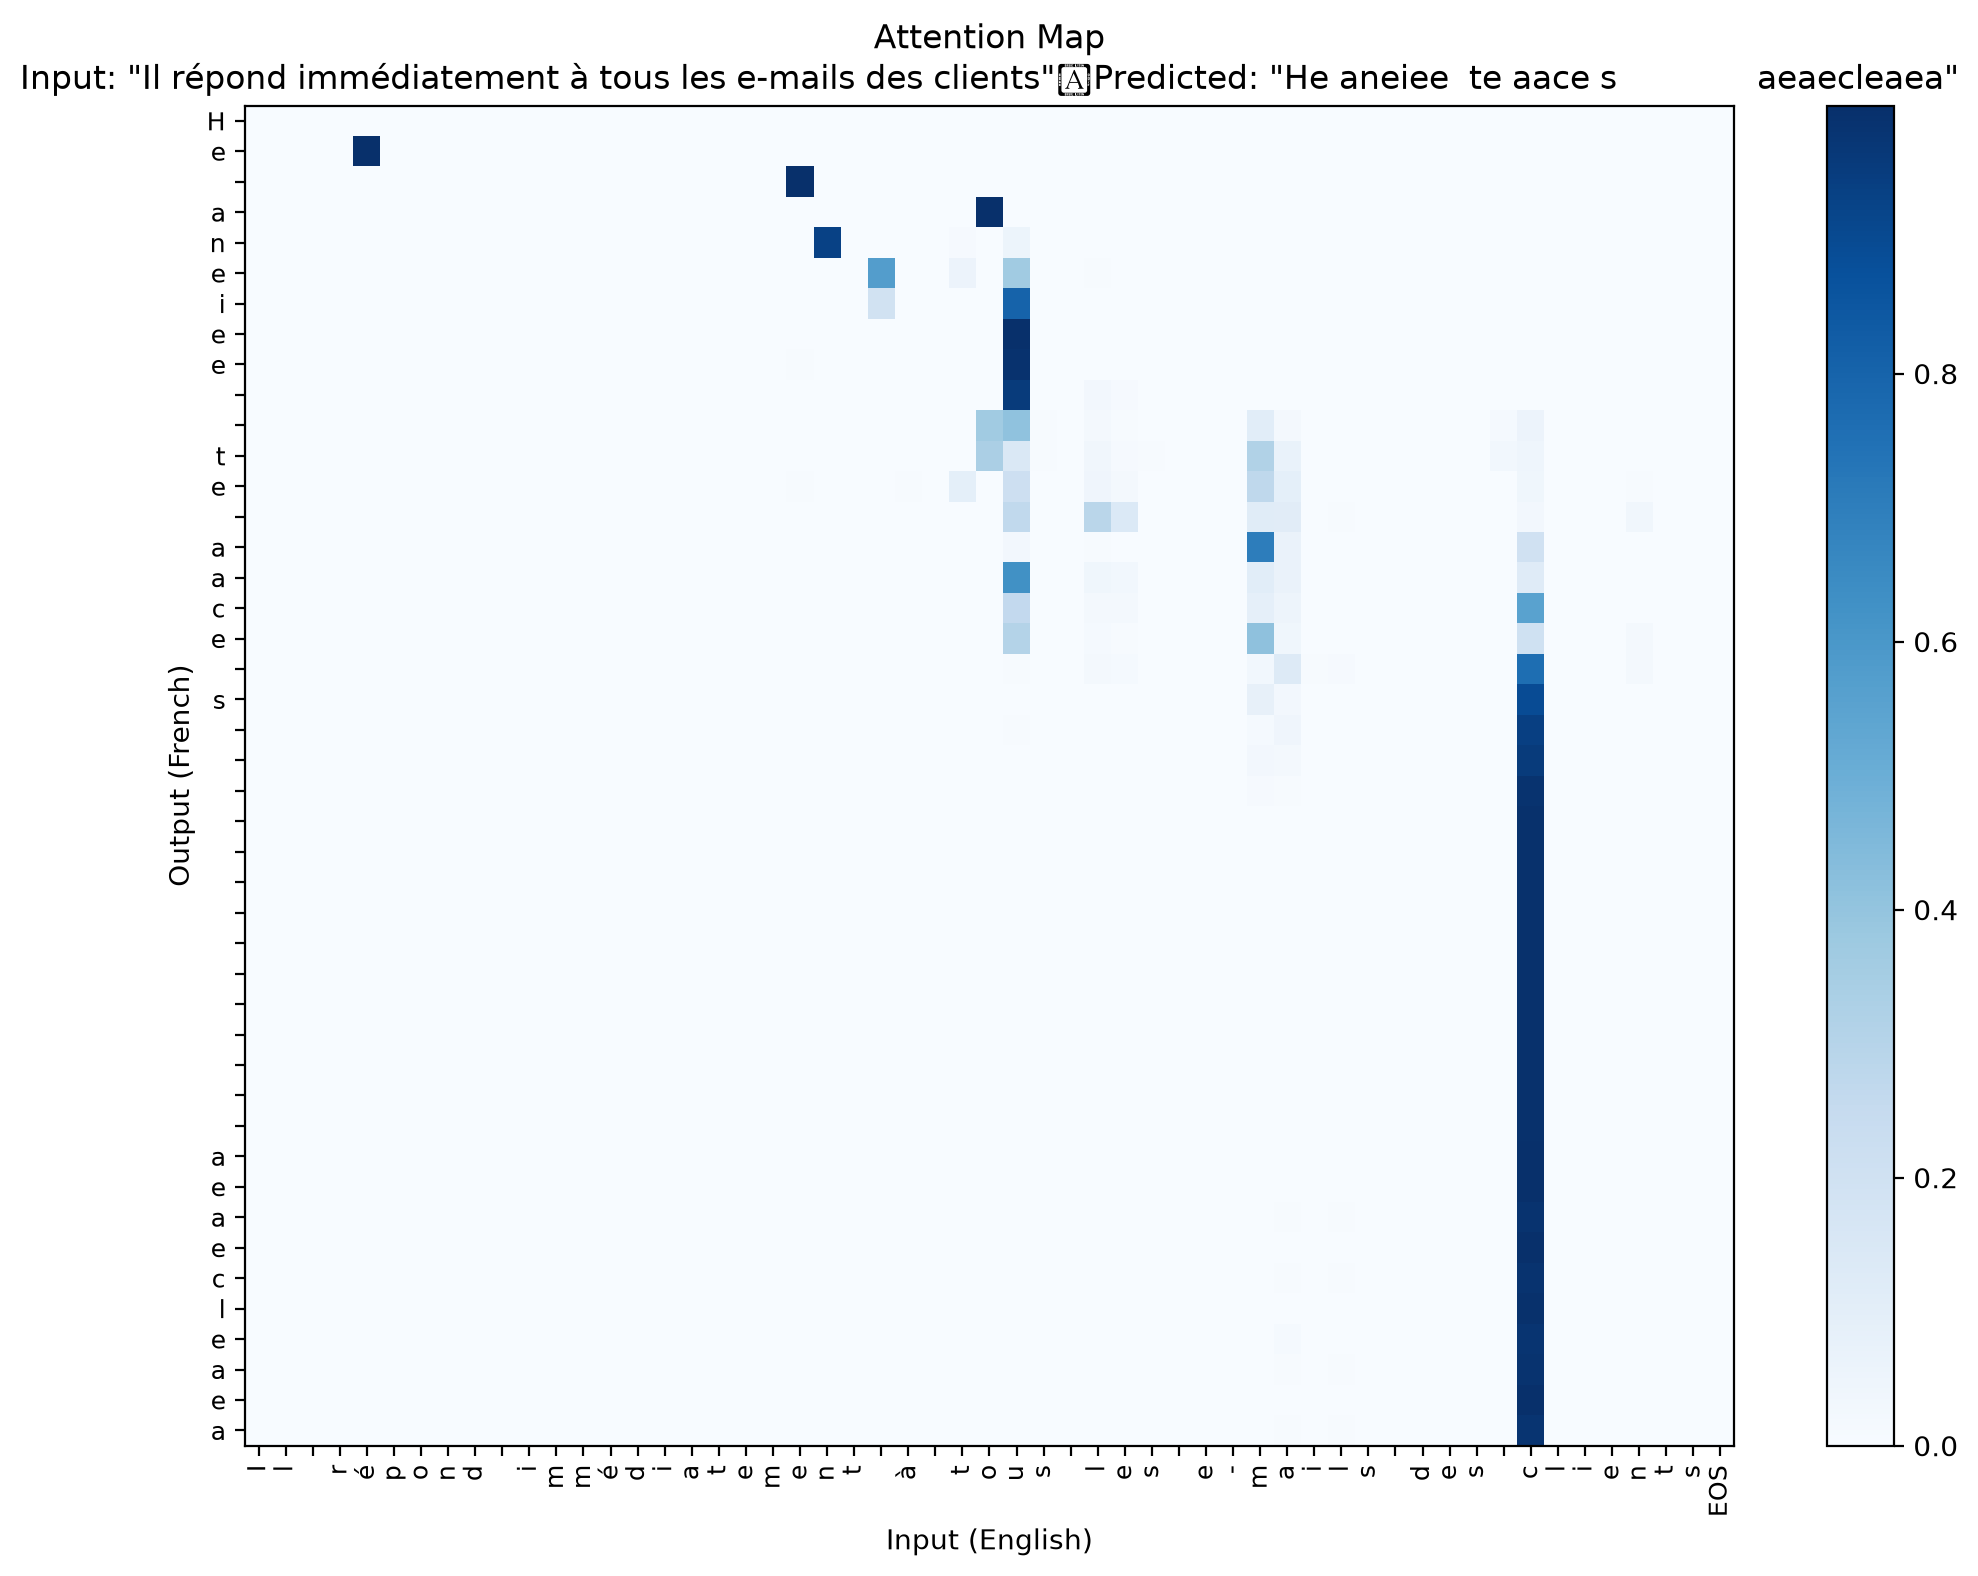
\includegraphics[width=\linewidth]{../../hw3/output/p3/attn_map_1.png}
    \caption{\textbf{Attention Map for French-to-English Translation with Attention}}
    \label{fig:reversedAttnMap1}
\end{figure}

\begin{figure}[H]
    \centering
    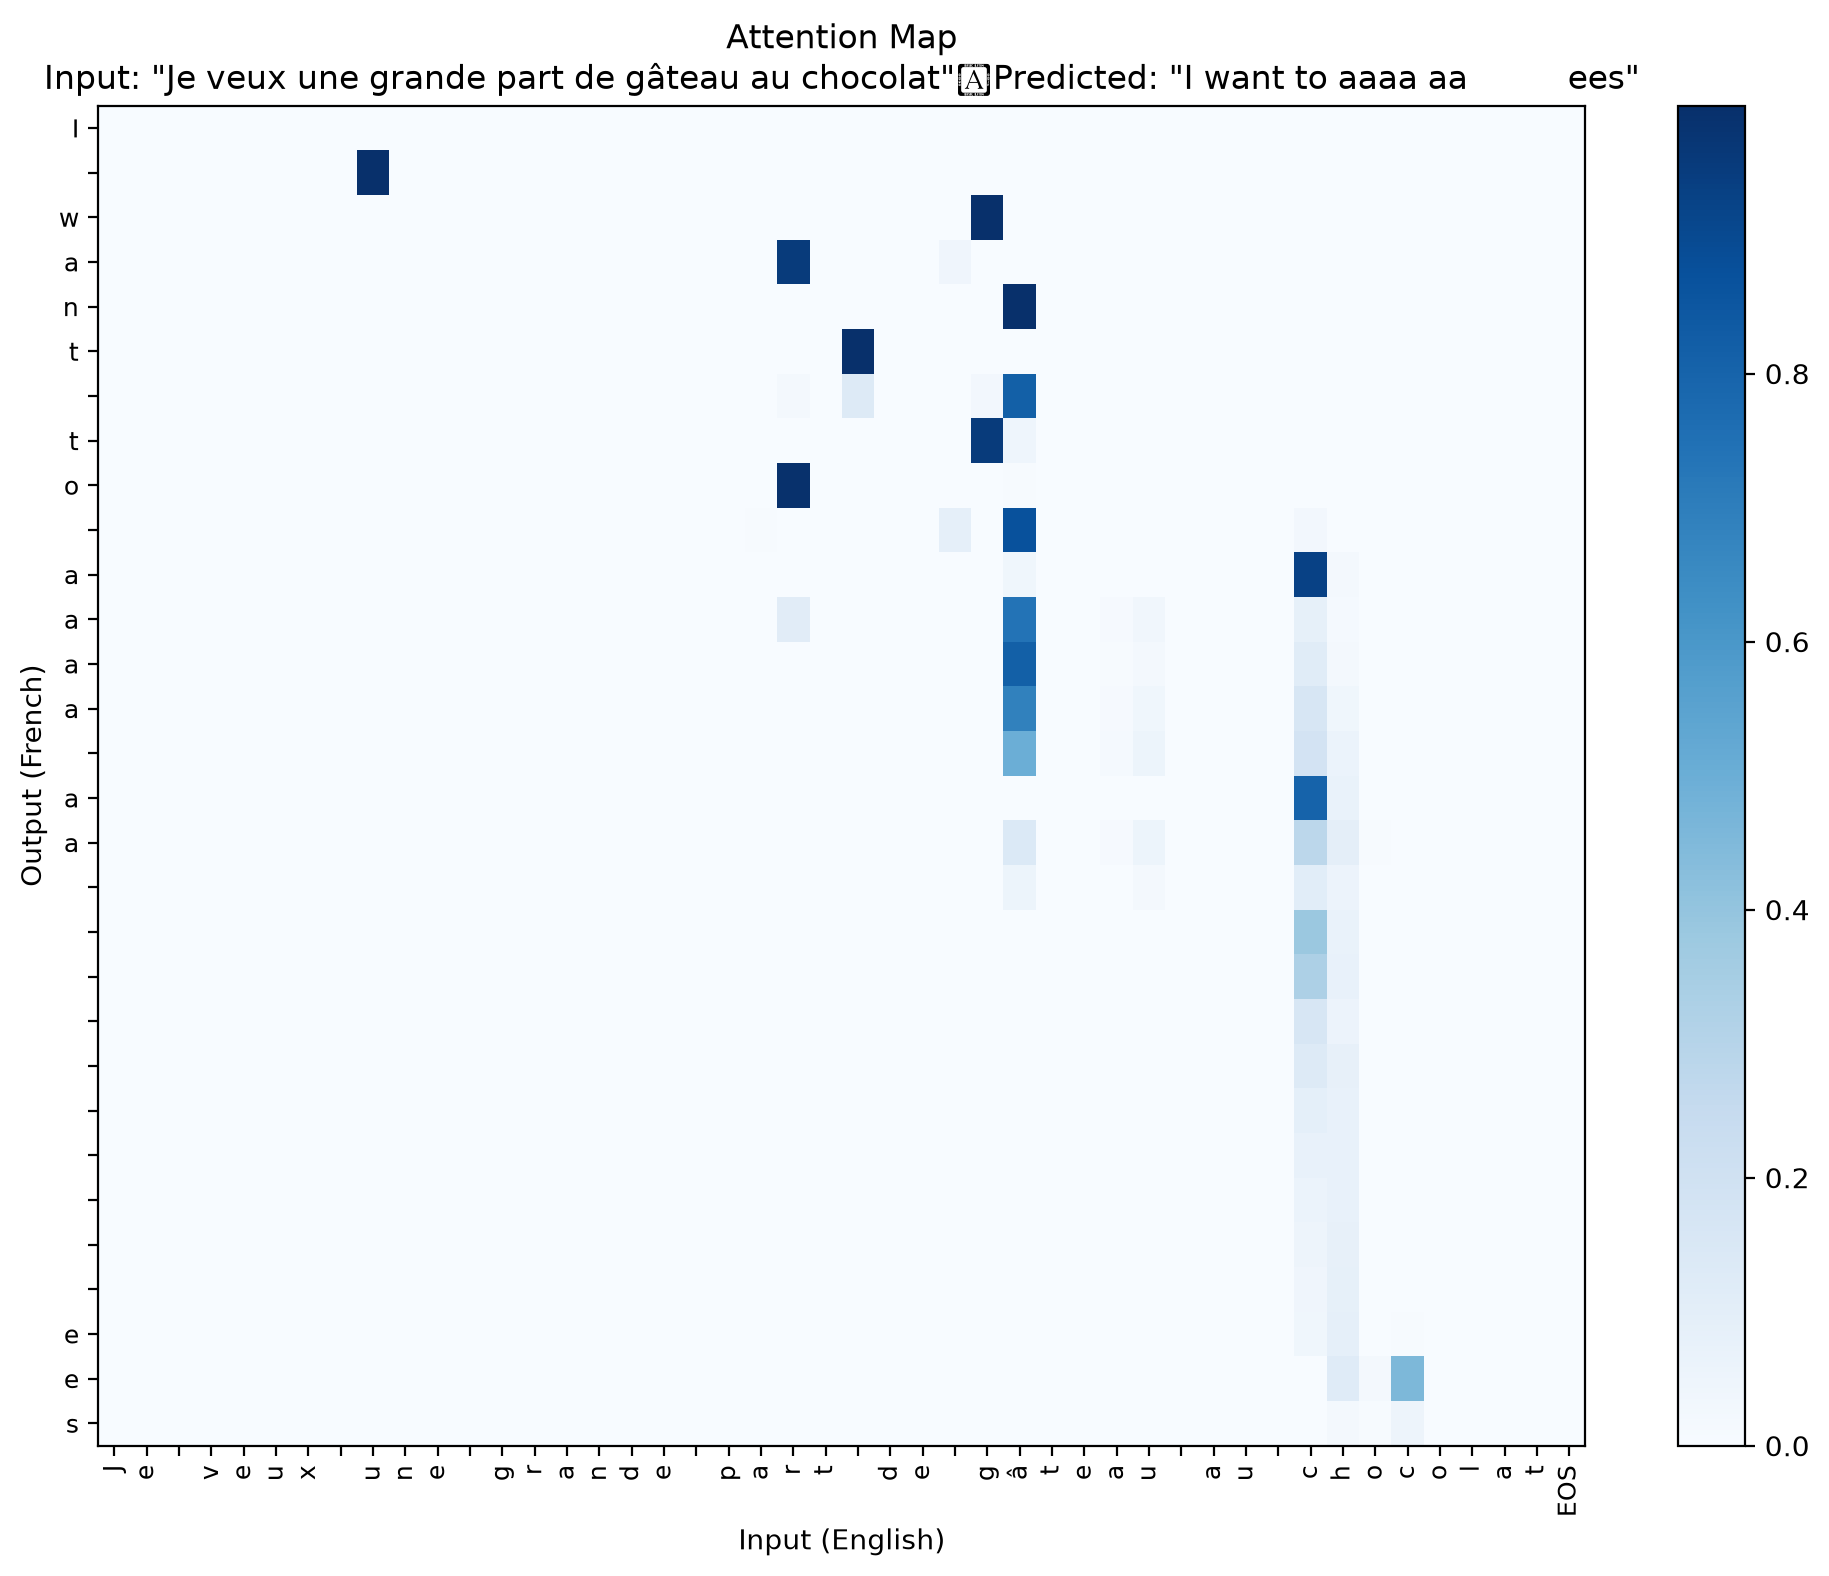
\includegraphics[width=\linewidth]{../../hw3/output/p3/attn_map_3.png}
    \caption{\textbf{Attention Map for French-to-English Translation with Attention}}
    \label{fig:reversedAttnMap3}
\end{figure}

One significant thing to note is that the new attention maps for the reversed dataset show that the network had a easier time to pickup on context and relevant characters to look out for. The maps are more populated and we see a more emergent and prominent diagonal pattern.

\section*{\textbf{Synthesis Discussion}}
Based on the qualitative tests, evaluation curves, and attention maps plotted. I think translating from French to English is easier for the network to optimize. While this metric was not formally measured, when all the models are run at the same time, the network trains the baseline model on the reversed dataset faster than the original dataset which seems to imply that the network has an easier time learning and making connections between the sentences. Furthermore, the evaluation curves seem to indicate the networks trained on the reversed dataset, for the exact same hyperparameters, overfit less which means that the network is learning more trying to translate in that direction compared to English-to-French. The attention maps produced by the original and reversed datasets also seem to indicate the latter network has an easier time forming connections between the two languages than the former network. Also, the BLEU scores for the network, when trained with attention, show a notable improvement when the model tried to translate French sentences to English compared to the other way around. One discrepancy is the original baseline network having a higher BLEU score than the reversed dataset baseline network. However, this is just an outlier when comparing it to other metrics. Overall, I think the reason why the network has an easier time to translate from French to English is because English is the simpler language and so the network has an easier time comprehending how to form the translated sentence.

\end{document}